%페이지 세팅
\documentclass[11pt,a4paper]{article}
\setlength{\parindent}{0em}                  %DISTANCIA SANGRÍA
\setlength{\parskip}{0.5em}                  %DISTANCIA ENTRE PÁRRAFOS
\textwidth 6.5in
\textheight 9.in
\oddsidemargin 0in
\headheight 0in

\usepackage{amsmath}
\usepackage{tcolorbox}
\usepackage{amssymb}
\usepackage{amsthm}
\usepackage{lastpage}
\usepackage{fancyhdr}
\usepackage{accents}
\usepackage{setup}
\usepackage{import}
\usepackage{fancyhdr}
\usepackage{layouts}
\addtolength{\voffset}{0mm}
\addtolength{\textheight}{0mm}

\usepackage{xcolor}
\usepackage{mdframed}
\usepackage[shortlabels]{enumitem}
\usepackage{indentfirst}
\usepackage{hyperref}

\usepackage{enumitem}
\newlist{enumerateoptional}{enumerate}{1}
\setlist[enumerateoptional]{
    before=\let\item\optionalItem,
    label=\arabic*,
    nosep,
    labelindent=20mm,
    leftmargin=*
}
\let\realItem\item

\newcommand\optionalItem[1][]{%
  \refstepcounter{enumerateoptionali}% increment the counter
  \realItem[\bfseries#1~\theenumerateoptionali)]%
}
% caption 업데이트 
% \usepackage{subcaption}
\renewcommand{\thesubsection}{\thesection.\alph{subsection}}

% 여기서 변경하는 제목들을 설정해 준다. 
%%
%----------------- 예비레포트 주차 
\newcommand{\numnum}{1}
%-----------------단원명
% \newcommand{\SUBJECTT}{}
%-----------------문제번호들
% \newcommand{\problemnuma}{1}
% \newcommand{\problemnumb}{2}
% \newcommand{\problemnumc}{3}
% \newcommand{\problemnumd}{4}
% \newcommand{\problemnume}{5}
% \newcommand{\problemnumf}{6}
% \newcommand{\problemnumg}{7}
% \newcommand{\problemnumh}{8}
% \newcommand{\problemnumi}{9}

% Enumerate Listing modified 
\renewcommand{\labelenumi}{Problem  \theenumi}
\newcommand{\soln}[1][Answer]{\noindent\textbf{#1}\quad}

\newenvironment{problem}[2][Problem]  
    { \begin{mdframed}[backgroundcolor=gray!20] \textbf{#1 #2} \\}
    {  \end{mdframed}}

\begin{document}
\pagestyle{fancy}
\fancyhf{}
    \rhead{\small \textbf{2조} \quad 2016142096 \textbf{조윤신} \quad 2017142043 \textbf{김재민}}
    \lhead{Result Report Week \numnum}
\cfoot{\thepage}
\renewcommand\headrulewidth{0.3mm}
%\renewcommand\footrulewidth{0.3mm}
\thispagestyle{plain}

\begin{flushleft}
\textsc{School of Electrical and Electronic of Enginnering} \\
\textsc{eee 4474-01 : Experiments on Communication Networks }\\[0.1cm]
\small{\textsc{\textbf{2조} \quad 2016142096 \textbf{조윤신} \quad 2017142043 \textbf{김재민}}}\\

\end{flushleft}
\begin{flushright}\vspace{-25mm}
    
\includegraphics[height=3cm]{image/1.jpg}
    \vspace{5mm}
\end{flushright}
    \begin{center}\vspace{-1.5cm}
        \textbf{\huge  Result Report Week \numnum}\\ 
        \vspace{0.6mm}
        {\large Introduction to Wireshark}\\           
    \end{center}
    
\vspace{-5mm}
\rule{\linewidth}{0.4mm}
\vspace{-5mm}
% main documents

%%%%%%%%%%%%%%%%%%%%%%%%%%%%%%%%%%%%%%%%%%%%%%%%%%%%%%%%%%%%%%%%%%%%%%%%%%%%%%%%%%%%
\import{./week01}{01_exp1}

\import{./week01}{02_exp2}

\import{./week01}{03_exp3}
\end{document}


% 사진을 첨부하는 포멧 
%%%%%%%%%%%%%%%%%%%%%%%%%%%%%%%%%%%%%%%%%%%%%%%%%%%%%%%%%%%%%%%%%%%%%%%%%%%%%%%%%%%%
    Bla Bla 1\\*
%
         \vspace{-4mm}
        	\begin{figure}[!h]
        		\centering
        			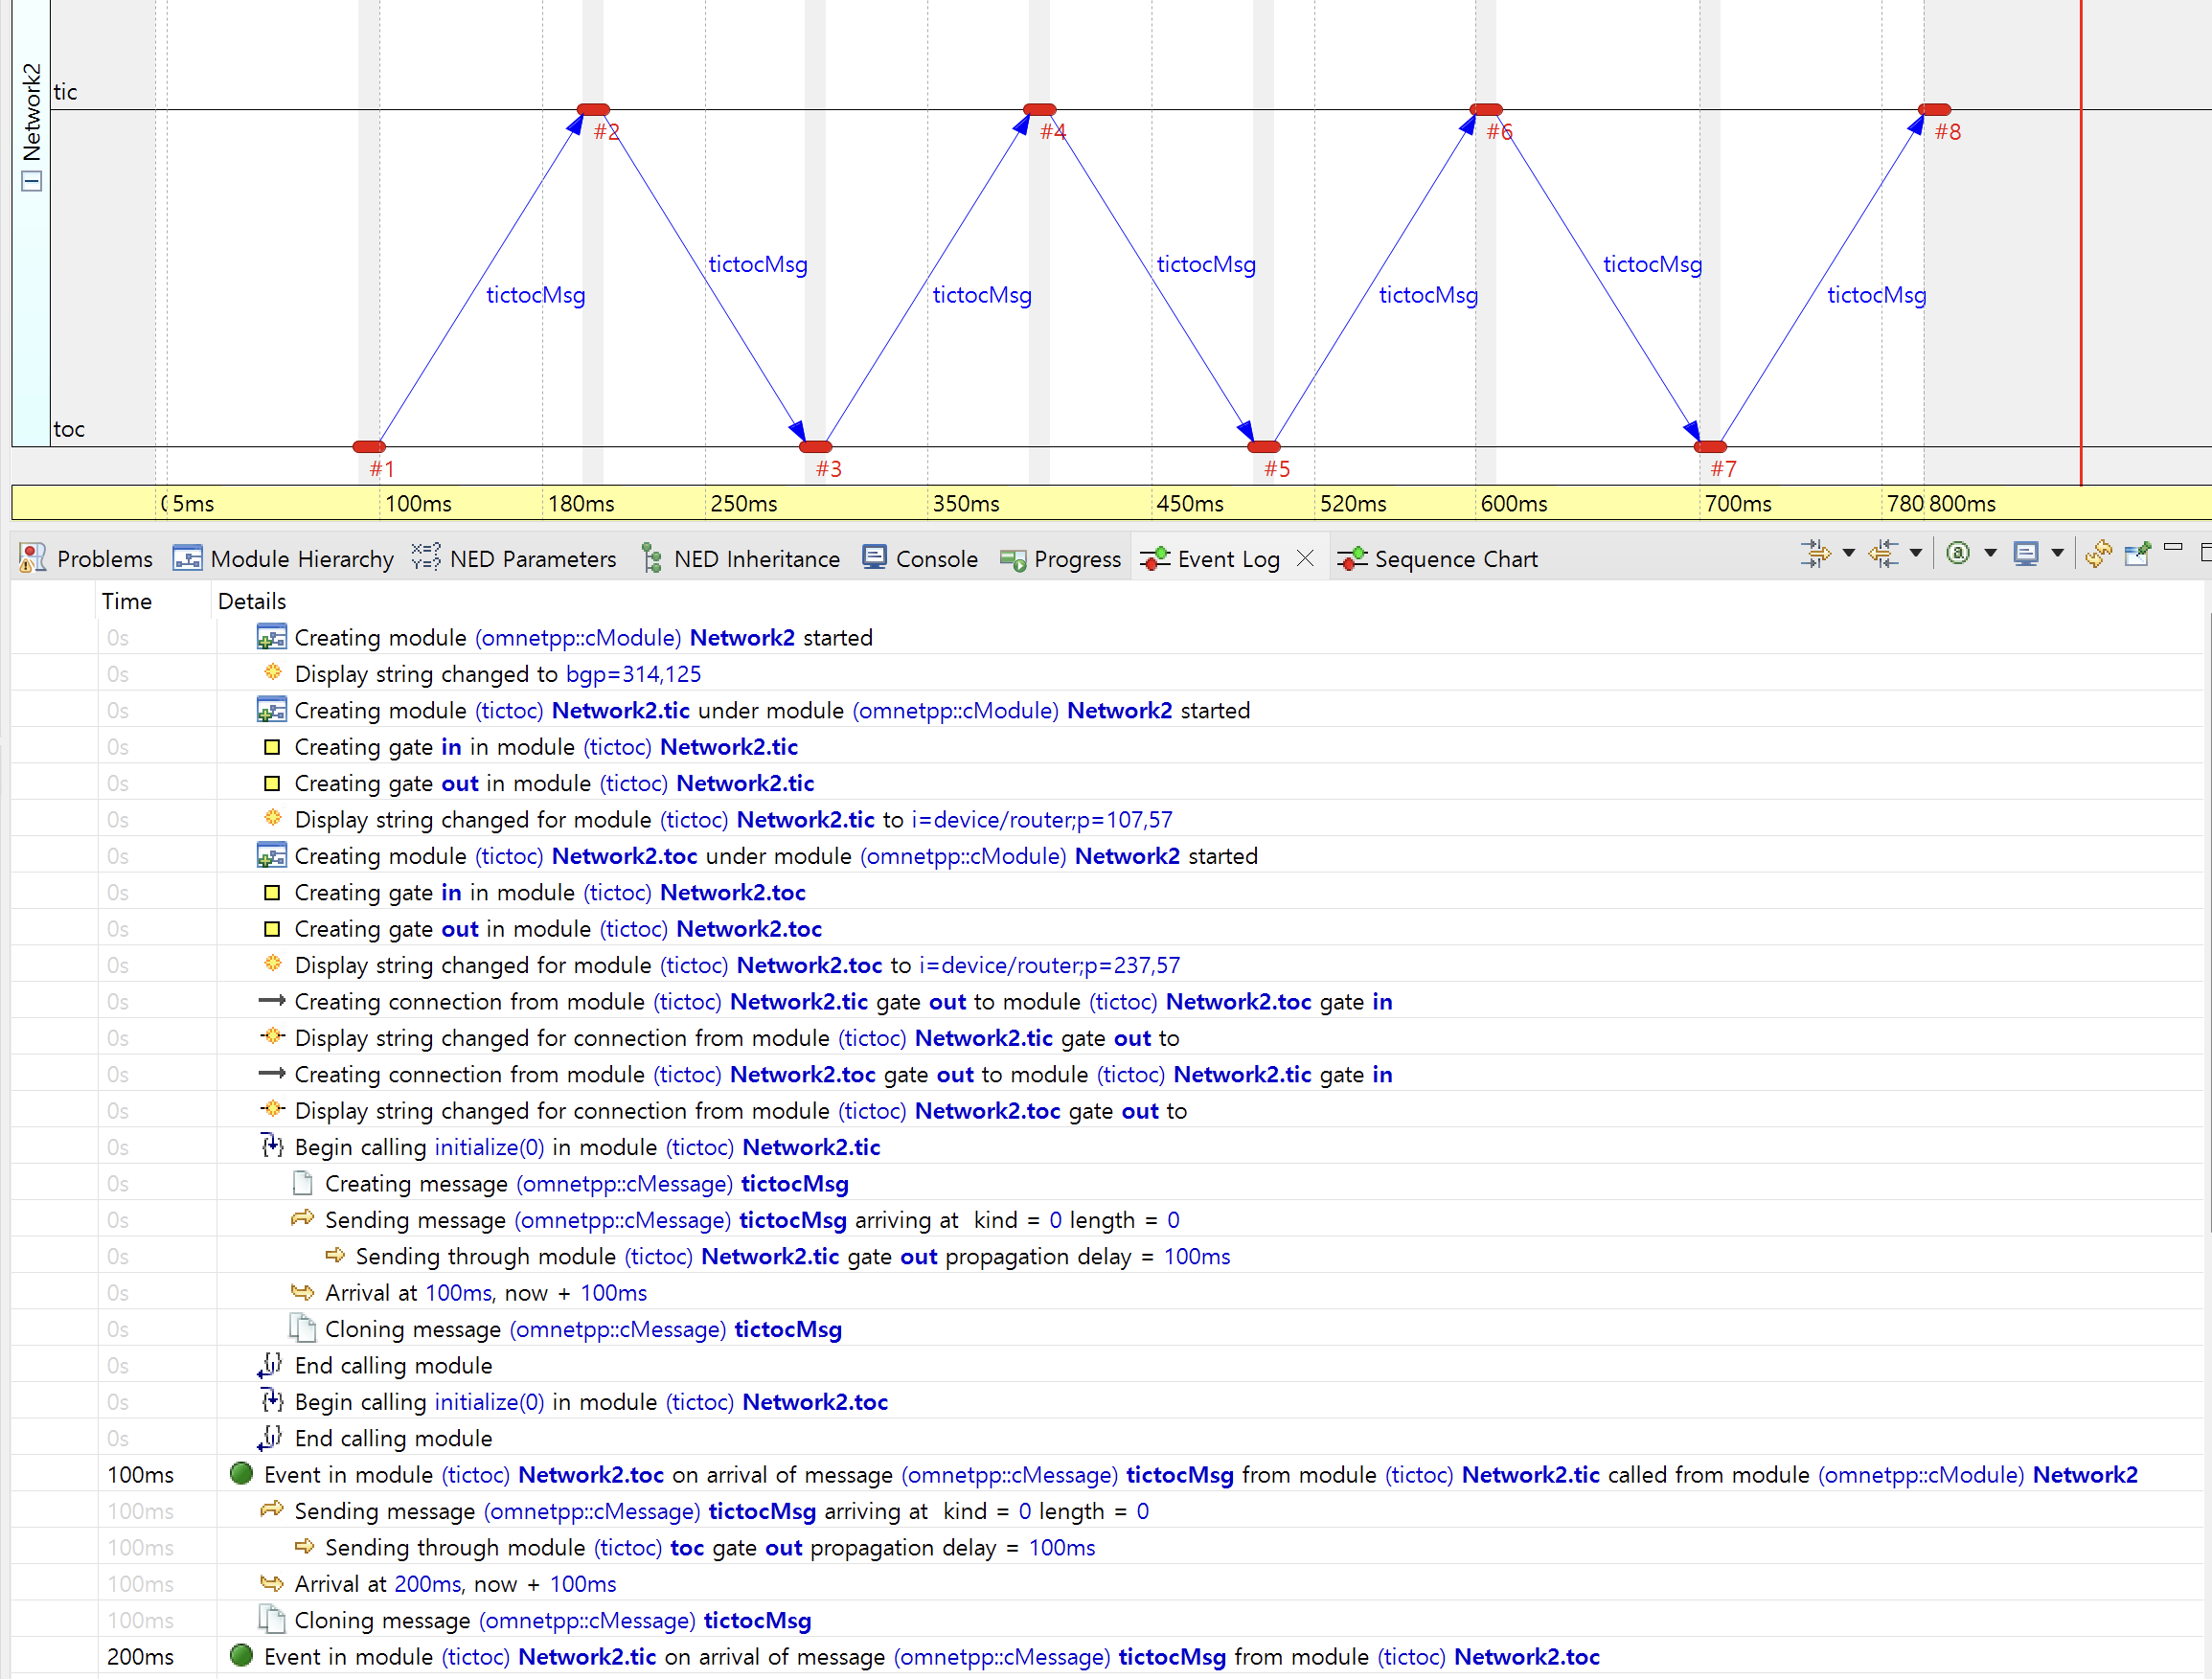
\includegraphics[width=.4\textwidth]{image/2-2.png}
        			\caption{Experiment 1 - top.v}
        	\end{figure}
        \vspace{-4mm}  
%

\vspace{-3mm}
    Bla Bla 2 
%%%%%%%%%%%%%%%%%%%%%%%%%%%%%%%%%%%%%%%%%%%%%%%%%%%%%%%%%%%%%%%%%%%%%%%%%%%%%%%%%%%%%%%%%%